Based on PATO, we conduct a series of experiments. To examine the
feasibility of using a single ontology to support multiple different
program analyses efficiently, we implement four types of program
analysis on PATO: canonical loop analysis, control flow graph
construction, data access pattern analysis, and GPU data placement
guidance. They differ in domains, relations, scopes, and intended
usage. Using GPU data placement optimization, we examine whether
ontology can indeed enable seamless linkage of various sources of
knowledge (programs, domain experts, and hardware) and whether
ontology-based program analysis can actually help guide program
optimizations. Using the liveness analysis on two compilers
(ROSE~\cite{ROSE} and LLVM Clang~\cite{Lattner2004}), we
examine the easiness of ontology for promoting cooperations among
different analysis tools. We next report our observations in each of
the experiments.

For the interest of space, our description concentrates on the 
canonical loop analysis and the GPU data placement guidance,
and briefly covers the other two program analyses.

%%%%%%%%%%%%%%%%%%%%%%%%%%%%%%%%%%%%%%%%%%%%%%%%%%%%%%%%%%%%%%%%%%%%%%%%%%%%%%%
\subsection{Canonical Loop Analysis}
%\TODO{description based on the Page5 rightside and P6 leftside of the
%  previous version (main\_ws.pdf); clarity needs to be improved; add the part on
%  iterators to show the easy tool-human synergy allowed by the new
%  paradigm}

%We use canonical loop analysis as the first example to evaluate the benefits of PATA. 
To help readers get a concrete understanding of using logic programming
for ontology-based program analysis, we first explain the Prolog code
for canonical loop analysis in a certain degree of detail. 

As mentioned earlier, canonical loop analysis (CLA) checks whether a
loop is in a predefined canonical form.  CLA is a fundamental analysis
to enable various loop
optimizations~\cite{kandemir1999improving,LiaoSemantic-aware2010,DaMata2013}.
%There are different specifications of what a canonical loop should
%look like.
In particular, we use the \emph{canonical loop form} defined in the OpenMP specification \cite{openmp13} as an example, shown in Figure~\ref{fig:canonical}.  
The specification of an OpenMP canonical loop can be written as declarative Prolog rules as shown in Listing~\ref{code:iscl}.
We use italic font to distinguish variable from normal symbols.

\begin{comment} % redundant figure, remove it
\begin{lstlisting}[xleftmargin=.1\columnwidth,xrightmargin=.1\columnwidth,
caption=Specification of an OpenMP canonical loop, label=code:cldef]
  for (init-expr; test-expr; incr-expr) structured-block
% init-expr is one of:
var = lb
integer-type var = lb
pointer-type var = lb
...
\end{lstlisting}
\end{comment}
%where every loop component has detailed specification (shown in Figure~\ref{fig:canonical}) .
%The above specification can be mapped to the logic rule of
%\begin{equation*}
%\begin{split}
%\text{is-a(canonical loop)} & := \text{has-a(inti-expr)} \wedge \text{has-a(test-expr)} \\ 
% & \wedge \text{has-a(incr-expr)} \wedge \text{has-a(block)}
%\end{split}
%\end{equation*}

\begin{lstlisting}[basicstyle=\ttfamily\footnotesize,
float=h, caption={Prolog specification of an OpenMP canonical loop
(italic upper-case for variables, lower-case for properties)},
escapechar=@, 
 label=code:iscl]
% top level rule to find canonical loop
canonicalLoop(@\emph{Loop}@) :- 
 isForStatement(@\emph{Loop}@), !, %'!' prevents backtracking
 hasForInit(@\emph{Loop}@, @\emph{InitExpr}@), %',' means logic AND
 canonicalInit(@\emph{InitExpr}@, @\emph{LoopVar}@),
 hasForTest(@\emph{Loop}@, @\emph{TestExpr}@),
 canonicalTest(@\emph{TestExpr}@, @\emph{LoopVar}@),
 hasForIncr(@\emph{Loop}@, @\emph{IncrExpr}@),
 canonicalIncr(@\emph{IncrExpr}@, @\emph{LoopVar}@),
 (
  hasType(@\emph{LoopVar}@, 'IntType'); %';' means logic OR 
  hasType(@\emph{LoopVar}@, 'PointerType')
 )
 hasBody(@\emph{Loop}@, @\emph{ForBody}@),

% supportive rules to find canonical init-exp 
canonicalInit(@\emph{Init}@, @\emph{LoopVar}@) :-
 hasOperator(@\emph{Init}@, @\emph{AssignOperator}@), !,
 hasLeftOperand(@\emph{AssignOperator}@, @\emph{VarRef}@),
 referTo(@\emph{VarRef}@, @\emph{LoopVar}@),
 hasRightOperand(@\emph{AssignOperator}@, @\emph{LB}@).

% rules with same heading: combined using logic OR
canonicalInit(@\emph{Init}@, @\emph{LoopVar}@) :-
 hasVarDecl(@\emph{Init}@, @\emph{LoopVar}@), 
 hasInitializer(@\emph{Init}@, @\emph{Initializer}@),
 hasValue(@\emph{Initializer}@, @\emph{LB}@),	
% the rest is omitted ...
\end{lstlisting} 

In the Prolog specification, the \emph{head}
\textsf{cannonicalLoop(Loop)} asks for individuals that satisfy all
clauses in the \emph{body}.  The (\textsf{,}) plays the role of logic
conjunction (AND operation).  Every clause in the \emph{body} is
deducted by its own rule.  In the end, the deduction is backed by
queries on the existing knowledge base.  The
\textsf{isForStatement(Loop)} is a more readable wrapper of the
ontology query \textsf{Loop is-a ForStatement}, where the variable
\textsf{Loop} binds to individuals if ontology triples
\textsf{(some-loop is-a ForStatement)} exists in the knowledge base.
Once the Loop is bound to some individual, clauses like
\textsf{hasForInit(Loop, InitExpr)} search the knowledge base for
\textsf{(some-loop hasForInit some-init-expr)} triples.  Then
\textsf{canonicalInit(InitExpr, LoopVar)} checks if the found
initial expression individuals conform to the language specification.
The query also returns the loop variable \textsf{LoopVar} if it can
find it.

The analysis further checks whether the loop's init construct conforms
to the specification.
%They checks if the initial expression of the loop conforms to the specification and also return the loop variable \textsf{LoopVar}. 
%The code is declarative and self-explained. 
The first rule handles the \textsf{var = lb} style while the second
rule deals with other styles.  Different rules with the same head name
form the logic disjunction (OR operation).  The \emph{cut} operator
(i.e., the ! symbol) is used to prevent unwanted backtracking.  It
means that, as long as the first rule matches the form
\textsf{hasOperator(Init, AssignOperator)}, there's no need to check
the second rule of the variable declaration form.
%Again, every clause in the body can be grounded to queries on the knowledge base. 
Line 11 to 12 are the rules to do the type checking of loop variables.
The \textsf{(;)} means logic disjunction (equivalent to two separated rules).

\vspace*{.1in}\noindent {\bf Experimental Results} 

%\TODO{report comparison (lines of source code, analysis time, etc.)}

The ontology in PATO successfully supports the analysis.  We compare
it with the imperative implementation in the ROSE compiler. The
algorithm in ROSE traverses the AST tree of a program to find {\em for}
statement nodes and check whether their sub-tree are in the canonical form.
The code is written in C++ and highly dependent on the ROSE AST's
internal data structures.  The time complexity is $\mathcal(O)(n)$,
where $n$ is the number of AST nodes.  

The code length of PATO-based analysis is about half of the imperative
implementation in the ROSE compiler (190 versus 380 lines).  We
compare their analysis time on a machine equipped with Intel Core-i5
CPU of 3.2GHz and 8GB DRAM. We use the NAS Parallel Benchmarks
(NPB)~\cite{Bailey91thenas} for the measurement.

\begin{comment} % this table takes too much space and show some info. too early. using text instead for each analysis
\begin{table}[t]
\centering
\begin{tabular}{l|lll}
\hline
Analysis & PATO & ROSE & Clang \\
\hline\hline
CLA & 190 & 370 & - \\
CFG & 400 & 1200 & 3500 \\
DAP & 180 & - & 2000 \\ 
\hline
\end{tabular}
\caption{Comparison of lines of source code.}
\label{tbl:loc}
\end{table}
\end{comment}

The results are shown in Figure~\ref{fig:npb-cl}.  The frontend time
corresponds to the parsing time of the \emph{parser} in
Figure~\ref{fig:pato}.  PATO uses the same frontend as the ROSE
implementation.  The time of program knowledge generation (KB gen.)
represents the time of the ontology translator/converter in the PATO
framework.
%It doesn't include the frontend time.
Finally, the other two bars are the time of the canonical loop
analysis with PATO and ROSE respectively.

For the canonical loop analysis alone, we can see that the PATO
declarative approach even beats the native implementation for most
cases.  It is slower only when the line number is small.  One reason
is that the ROSE's imperative implementation traverses
the whole AST tree to find all for loops.
%and the time complexity is in $O(n)$. 
For PATO's declarative implementation, the \textsf{isForStatement}
relation information is stored explicitly and can be efficiently
accessed by the hash-indexed keyword implementation of Prolog.
%all relational triples \textsf{subject relation object} are hash-indexed by all \textsf{subject, relation, object} keywords. 
%So in Listing~\ref{code:iscl}, when we use \textsf{isForStatement(Loop)} to query the knowledge base, the \textsf{Loop} is narrowed down to only the \emph{for-loop} in $O(1)$ time and the processing of every \emph{for-loop} instance can be regarded as $O(1)$. 

The ontology-based declarative analysis does have an obvious overhead:
It needs an extra step to traverse the AST tree and build the initial
knowledge base.  However, as shown in the figure, the overhead is
relatively smaller than the frontend time.  Besides, for the PATO
system, the generated knowledge base can be reused for different
program analyses (e.g., the control flow graph analysis
later). 

\begin{figure}[h]
\centering
	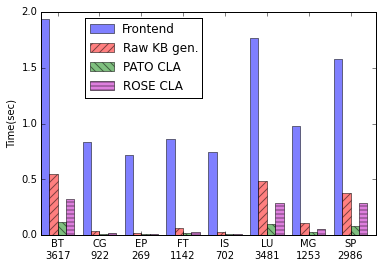
\includegraphics[width=.6\columnwidth]{graph/npb-cl.png}
	\caption{Time comparison of the canonical loop analysis. The
          X-axis shows the benchmark names and their numbers of
          source-code lines.}
	\label{fig:npb-cl}
\end{figure}


%Another advantage of the declarative approach is that the analysis rules can be added incrementally. To handle different cases for the same definition, we just need to add more rules without changing the existing ones. 
%It is seen that writing rules for program analysis is very productive in adding language feature support. 
%To cover more cases, we just need to add more rules in a very modular way. 
\noindent{\em Extensibility.} An appealing property of using ontology
is the good extensibility. The previous discussion only covers
canonical loops in C programs using primitive loop variable types,
such as pointer and integer types.  OpenMP allows C++ canonical loops
using complex iterator types for loop variables.
%For example, in the canonical loop specification, the \textsf{var} can be a variable of type random access iterator for C++. 
The iterator type must support random access---that is, allowing
element accesses using an arbitrary offset position relative to the
element they point to (offering a functionality similar to pointers).
%The random access iterator is an iterator that supports the access to elements in any order. 
%It provides 
%operations of ordinary C pointer arithmetic. 
Examples of random access iterators include \textsf{std::vector<T>::iterator} and \textsf{std::deque<T>::iterator}. % and ordinary pointers. 
Also, programmers often define their own random access iterators. 
%To support the CLA for C++, the analysis tools need to be able to recognize random access iterators. 
A conventional solution to extend an imperative CLA implementation is to store the known random access iterators, including the custom-defined ones, into a container for the compiler implementation to look-up. 
The solution is ad-hoc and it is not easy to exchange this knowledge with other tools or developers.

Ontology-based program analysis allows easy extensibility. 
In PATO, we can easily add the concept \textsf{RandomAccessIterator} in the language ontology and describe it logically as $\mathsf{is-a(Iterator)}\wedge\mathsf{has(RandomAcess)}$. 
The knowledge of \textsf{is-a(Iterator)} property can be gained by the knowledge builder while the knowledge \textsf{has(RandomAcess)} can be inserted into the knowledge base using the standard OWL API, either automatically by tools or manually by developers. 
The analysis rules can reason about the random access iterator logically. 
All the resulting ontology can be then shared and reused by different analyses.

\subsection{Control Flow Graph Construction}

The second program analyses we have developed on PATO is control flow
graph (CFG) construction. Different from the canonical loop analysis,
it requires the examination of control flows of the whole program.  On
PATO, it can be easily done through the set of simple rules.  by
following the algorithm of inductive graph
constructions~\cite{fischer_crafting_2009}.  The construction is
intuitive. For example, the rule to construct the CFG of a
\textsf{while}-statement is shown in Listing~\ref{code:cfg-prolog}.
\begin{lstlisting}[xleftmargin=.1\columnwidth,
xrightmargin=.1\columnwidth, escapechar=@, 
caption= Rule to construct CFG for a While statement, label=code:cfg-prolog]
cfg(@\emph{Stmt}@, @\emph{Entry}@, @\emph{Exit}@) :-
 isWhileStatement(@\emph{Stmt}@), !,
 hasCondition(@\emph{Stmt}@, @\emph{ConditionStmt}@),
 hasBody(@\emph{Stmt}@, @\emph{BodyStmt}@),
 @\emph{Entry}@ = @\emph{ConditionStmt}@,
 @\emph{Exit}@ = exit(@\emph{Stmt}@),
 cfg(@\emph{BodyStmt}@, @\emph{BodyEntry}@, @\emph{BodyExit}@),
 makeTrueEdge(@\emph{ConditionStmt}@, @\emph{BodyEntry}@),
 makeFalseEdge(@\emph{ConditionStmt}@, @\emph{Exit}@),
 makeEdge(@\emph{BodyExit}@, @\emph{ConditionStmt}@).
\end{lstlisting}

%This construction rule constructs CFG on per-statement level. 
The first clause in the body matches this rule with only the \textsf{while}-statement. 
The rest clauses find different components of the \textsf{while}-statement and construct the CFG nodes and edges. 
%according to Figure~\ref{fig:cfg}. 
%It is seen the process is very intuitive. 
A blank node (\textsf{exit(Stmt)}) is created to represent the exit node for the \textsf{while}-statement. 
The inductive construction for nested body statements are implemented by the recursive CFG rule \textsf{cfg(BodyStmt, ...)}.
%The per-statement CFG can be converted to basic block based CFG and the temporary blank nodes are removed. 
%\TODO{How to convert to basic block? Show the rules please.}
%Rules for different kind of statements are implemented separately and match the correct statements automatically.
The resulting CFG graph can be explicitly stored in ontology. 
We define relations like \textsf{hasNextEdge} to represent the directed edge in the CFG.
Nodes of CFG are just existing language construct entities in the program ontology.

\vspace*{.1in}\noindent {\bf Experimental Results} 
%\TODO{\sout{report comparison (lines of source code, analysis time, etc.)}}
For CFG analysis, we reuse the same initial knowledge base (originally generated to support the canonical loop analysis). 
%This shows the advantage of ontology-based program analysis -- the knowledge is easily shared and reused. Thus the overhead of building the knowledge is amortized over different analysis.
We compare our PATO implementation with the implementations of ROSE and Clang~\cite{lattner2008llvm}. 
%Both ROSE and Clang provide source level CFG analysis in their code base. 
%\TODO{what CFG construction algorithms are used in two compilers? Are the comparable to PATO's algorithm?}
Both ROSE and Clang implementations use the similar inductive construction algorithm but the details are different, especially the internal data structures. 
%Besides, ROSE and Clang support C++ while PATO doesn't support for now.
%Due to the difference of compiler implementation, it is difficult to do a strict comparison of code length. 

For productivity, we only measure the core code of the CFG analysis itself. % not including any dependency calls. 
Our goal is to find that if a specific analysis was not provided by the compiler, how many lines of codes are needed to implement it based on the existing APIs of the compiler. 
Source code comments and CFG printing statements are also excluded as much as possible to make the comparison fair.  
%The approximate line numbers are shown in Row 2 of Table~\ref{tbl:loc}. 
It turns out that the declarative approach uses only 400 lines of code, which is up to 8.75X more efficient than the traditional compiler implementations (1200 and 3500 lines for ROSE and Clang respectively).

The performance comparison is shown in Figure~\ref{fig:npb-cfg}.  The
time for PATO analysis doesn't include the knowledge building time.
Similarly, the time for ROSE and Clang analysis doesn't include their
frontend time.  The speed of the PATO analysis is as competitive as
imperative approaches due to the efficient storage and query of our
knowledge base.
%\TODO{Why ROSE's CFG is slowest? Please comment}
\begin{figure}[h]
	\centering
	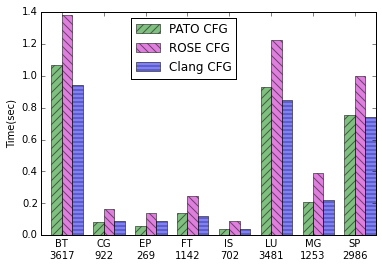
\includegraphics[width=.6\columnwidth]{graph/npb-cfg.png}
	\caption{Comparison of the analysis time taken by the three
          implementations for CFG construction.}
	\label{fig:npb-cfg}
\end{figure}

%%%%%%%%%%%%%%%%%%%%%%%%%%%%%%%%%%%%%%%%%%%%%%%%%%%%%%%%%%%%%%%%%%%%%%%%%%%%%%%
\subsection{Data Access Pattern Analysis}

%\TODO{One or two paragraphs to briefly explain what the analysis is and how it is implemented.}
The third analysis we have developed on PATO is data access pattern
analysis. Analyzing data access patterns is critical to many memory
optimizations (e.g., improving CPU cache
locality~\cite{kandemir1999improving}, enhancing GPU data
placement~\cite{Chen2014, Jang2011}.)  In our experiment, we
demonstrate how to use PATO to easily extract out data access patterns
from a CUDA (a GPU programming model from NVIDIA)~\cite{nvidia2011nvidia}
program.  Listing~\ref{code:dap-eg} shows an example
CUDA kernel executing a two level loop, where \textsf{f(tid,i,j)} is
an affine function about the thread index (\textsf{tid}) and loop
index. % (\textsf{i, j}).
\begin{lstlisting}[xleftmargin=.1\columnwidth,
xrightmargin=.1\columnwidth,
caption=An example CUDA kernel loop, label=code:dap-eg]
for(i=0;i<N;i++) {
 for(j=0;j<M;j++) {
  A[f(tid, i, j)]=B[...]+C[...]
 }
}
\end{lstlisting}

In this experiment, we define a data access pattern of an array as the
access expression (or called subscript expression) of that array in
each access, the lower and upper bounds of the loops surrounding the
accesses to that array, the number of reads and the number of writes
to that array, and the ranges of elements of the array being
accessed. Choosing such a definition is because a previous
work~\cite{Chen2014} has already implemented a C/C++ code in a
source-to-source compiler to extract the same set of
information. Using the same definition allows us to make a
head-to-head comparison.

Our experiment shows that with PATO, each of the types of
information can be easily extracted from the kernel code through just
a few lines of Prolog statements. For example, to obtain the index
range of arrays in a double nested loop as the arrays \textsf{A, B, C}
in Listing~\ref{code:dap-eg}, our query in Prolog is as follows:

\begin{lstlisting}[xleftmargin=.1\columnwidth,
xrightmargin=.1\columnwidth,escapechar=@, 
caption=An example query for finding data access patterns, label=code:dap]
accessPattern(@\emph{Array}@) :-
 arrayRef(@\emph{Array}@),
 inNestedLoops(@\emph{Array}@, @\emph{LoopList}@),
 getLoopTripCount(@\emph{LoopList}@, @\emph{LTCs}@),
 getIndex(@\emph{Array}@, @\emph{ArrayIndex}@),
 eval(@\emph{ArrayIndex}@, @\emph{LTCs}@).
\end{lstlisting}

The clauses in the query are high-level APIs provided by the PATO
framework. The first clause on the right hand side asks the reasoner
to find all instances in the ontology that belong to the class
\textsf{ArrayRef} (which is a defined concept in the ontology to
represent array references). The second clause checks each of those
instances to see whether it is in a nested loop. If so, it recursively
finds the enclosing loops from inner to outer and returns the loop
statements in the variable {\em LoopList}. The third clause stores the
loop trip counts (LTC) of those loops into {\em LTCs}---which can be
symbols or constants of the lower and upper bounds of the loop
indices. The fourth clause gets the array access expression, and the
final clause evaluates the expression with the loop trip counts info.
The support of symbolic manipulation in Prolog turns out to be handy
for this analysis. In rule~\ref{code:dap}, the LTC of a loop can be
evaluated using the symbolic expression feature of Prolog.  Assuming
the affine function in Listing~\ref{code:dap-eg} is $f(tid, i, j) = 64
* tid + 8 * i + j$.  If the thread number \textsf{nthreads},
\textsf{M} and \textsf{N} can be inferred, then the range of the
access is evaluated to concrete value.  Otherwise, the symbolic
expression ($64 * nthreads + 8 * M + N$) is captured for later use.
The knowledge of different access patterns are stored as normal
ontology triples like \textsf{(A hasAccessRange "(0,
  64*nthreads+8*M+N)")}.
%or \textsf{(A
%  hasAccess "written")}. 
%  \footnote{In practice, A is referred to by
%  IRI.}, which can be later easily queried.

%\TODO{How do you extract info. about read/write,  linear/stride/random using Prolog ?} 
%\vspace*{.1in}\noindent {\bf Experimental Results} 
%\TODO{report comparison (lines of source code, analysis time, etc.)}

%\subparagraph{Time performance comparison}
%\TODO{Time performance comparison is missing?} 

%\subparagraph{Productivity Comparison}
The previous imperative data access pattern
analysis~\cite{Chen2014} has more than 2000 lines of source code.
PATO, on the other hand, only needs 180 declarative rules to implement
the same analysis. We test both implementations on a set of GPU kernel code from the CUDA SDK (mentioned later) and
%(?? cite benchmark paper or URL ?? ). 
they get the same extraction results and take similar length of
analysis time. 
%The PATO version takes (??  more or less??) time than the imperative version does. 

%%%%%%%%%%%%%%%%%%%%%%%%%%%%%%%%%%%%%%%%%%%%%%%%%%%%%%%%%%%%%%%%%%%%%%%%%%%%%%%
\subsection{Data Placement Guidance}
%\TODO{Explain what the optimization is and how it is implemented in
%  this work in the rule-based and PORPLE approach; describe the
%  comparison with the previous PORPLE in terms of productivity and
%  extensibility when adding the support of a new type of memory; the
%  description can be based on the old 4.2; be more clear and concise.}
%se data placement optimization as an example to demonstrate the use of ontology-based analysis.
The fourth analysis also help test the promise of ontology-based
analysis for guiding program optimizations. The particular
optimization is called data placement optimization. It is to find the
suitable kinds of memory to place the data in a program. It is
important for devices with multiple types of memory having different
performance characteristics. An example is NVIDIA Graphic Processing
Units (GPU) as shown by previous studies~\cite{Chen2014, Jang2011}.
An important analysis to support the optimization is to find an
optimal placement strategy for a given program on a specific GPU.  We
define this analysis as {\em data placement guidance}.

This analysis needs not only the knowledge about the program (such as
data access pattern), but also hardware memory specifications in order
to make appropriate decisions.  In this study, we confirm that it is
natural to use ontology to express hardware knowledge as the knowledge
is just a set of attributes or relations of the different parts of the
device. Moreover, because both the program knowledge and the hardware
knowledge are represented in the standard three-tuple format, they can
be automatically linked into one single ontology to support auto
reasoning about data placement.

Previous work uses customized memory specifications.  For example, the
PORPLE framework \cite{Chen2014} features the memory specification
language (MSL) to communicate a memory system to compilers.
%The syntax of MSL for memory specification is shown in Listing~\ref{code:msl}.
%\begin{lstlisting}[caption=PORPLE MSL syntax, label=code:msl]
%memSpec ::= name id swmng rw dim size blockSize banks 
%latency upperLevels lowerLevels shareScope 
%concurrencyFactor serialCondition ; end-of-line
%\end{lstlisting}
Listing~\ref{code:msl} shows the syntax of MSL and an example
specification for the constant memory of Tesla M2075.

\begin{lstlisting}[basicstyle=\ttfamily\footnotesize, caption={PORPLE
      Memory Specification Language (? represents unknown attributes).}, label=code:msl]
% syntax 
memSpec ::= name id swmng rw dim size blockSize banks 
latency upperLevels lowerLevels shareScope 
concurrencyFactor serialCondition ; end-of-line
% an example 
constantMem 1 Y r na 64K  ? ? 360clk <cL2 cL1> <> die ? ... 
\end{lstlisting}
%which conforms to the syntax in Listing~\ref{code:msl} and interprets correspondingly.
%This specification provides the information about the device. 
The example specification represents the type of memory (constMem), a unique ID (in numbers),  whether the memory is software manageable (Y or N) and whether a GPU kernel can read or write the memory ("rw" filed). 
%The field “dim”, if not “?”, indicates that the spec entry is applicable only when the array dimensionality equals to the value of “dim”. 
The other fields indicate dimensionality, memory size, number of
banks, memory latency, and so on.  The disadvantage of MSL is that it is
only extensible for a new GPU with a similar architecture.  But for
new hardwares with new attributes not present in the MSL syntax, the
MSL syntax, as well as the ad-hoc parser requires significant
modification.

In the PATO system, the ontology representation is more generic and
extensible.  We don't need to design any specific syntax for hardware
knowledge.  Only new concepts and relations (or properties) in the
hardware domain need to be added. Figure~\ref{fig:gpu_onto}
illustrates part of the GPU ontology.
\begin{figure}[t]
	\centering
	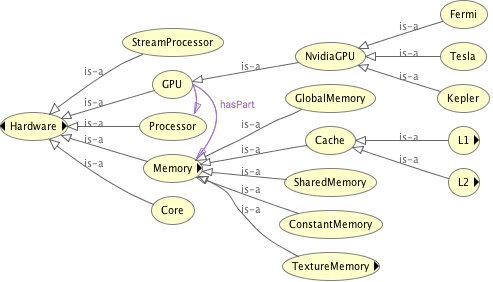
\includegraphics[width=.6\columnwidth]{graph/gpu_onto.jpg}
	\caption{Part of the GPU hardware ontology.}
	\label{fig:gpu_onto}
\end{figure}

Listing~\ref{ont:global_mem} shows the description of the
\textsf{Global Memory} on the Nvidia K20c GPU card.  The ontology
captures relations between the global memory and other components of
the GPU and also attributes of the memory.  It is expressive and easy
to extend. 
%In contrast, in PATO ontology representation, we just need to create new concepts for these new hardwares, new attributes and capture their relation with logic description.  
\begin{lstlisting}[xleftmargin=.05\columnwidth, 
xrightmargin=.05\columnwidth, float=h,
caption=Ontology of Tesla K20c global memory,label=ont:global_mem]
globalMem_k20c type GlobalMemory;
globalMem_k20c hasUpperLevel L2;
globalMem_k20c shareScope die;
globalMem_k20c pieces 1;
globalMem_k20c software_manageable true;
globalMem_k20c accessible "rw";
globalMem_k20c has_size 5032706048;
... % omitted
\end{lstlisting}

\vspace*{.1in}\noindent {\bf Guiding Data Placement}
Our experiment shows that with the ontology-based representation of
both program and hardware knowledge, it is easy to develop analysis to
guide the data placement optimization on GPU. 

Data placement guidance can rely on heuristic rules, mathematical
modeling, or their combinations.  For instance, a previous GPU
study~\cite{Jang2011} places data on GPU memory based on some
algorithms upon some empirical rules related with data access patterns
of arrays and the characteristics of different types of memory.  An
example rule is that constant memory is suitable for read-only data
which is small enough and satisfies the \emph{same address read}
condition (i.e., memory accesses to the array are the same across all
threads).  In another study named PORPLE~\cite{Chen2014}, analytical
cost models are used for finding good placements of data.  It
enumerates possible placement plans and estimates the cost of each
plan in terms of memory latency.  For each placement plan, it
coordinates all arrays together instead of placing them separately as
in the rule-based algorithm.
%PORPLE doesn't individually search for best memory for each array, but it considers all arrays and memories globally. 
%\TODO{wHAT does this mean? A single placement plan for all arrays?}

\begin{comment} % this looks too trivial to show in the paper
\begin{lstlisting}[caption=Top level rule for rule-based data placement, label=code:dp_rule]
suitablePlace(Array, Mem) :- 
 accessPattern(Array),
 suitableMem(Array, Mem). 
\end{lstlisting}
where the \textsf{getAccessPattern} is the rule of Listing~\ref{code:dap}. The \textsf{suitableMem} rule defines which memories are suitable for this array. 
\end{comment}

With PATO, it is easy to incorporate both the heuristic rules
and analytical models into an analysis for guiding data placement.
%This rule-based algorithm is straightforward to be implemented in PATO. 
For example, the logic rule to find suitable arrays for constant
memory can be expressed using Listing~\ref{code:dp_const}.
\begin{lstlisting}[xleftmargin=.05\columnwidth,
xrightmargin=.05\columnwidth,escapechar=@, 
caption=Rule for using constant memory, label=code:dp_const]
suitableMem(@\emph{Array}@, constantMem) :-
 readonly(@\emph{Array}@), 
 sizeFit(@\emph{Array}@, constantMem),
 sameAddressAccessWithinWarp(@\emph{Array}@).
\end{lstlisting}

Similarly, the algorithm used by PORPLE can be written as in
Listing~\ref{code:dp_model}.  The top-level rule \textsf{optimalPlace}
finds all the possible placement plans and estimates the cost of each
plan.  The \textsf{possiblePlacement} enumerates all possible plans.
(The rule-base placement algorithm (\textsf{suitableMem}) could be
plugged here to narrow down the search space.)  The estimation of the
cost of each placement is based on cache behaviors and is computing
intensive.  It is implemented as a {\em computable} (an external
procedure) and is hooked with the Prolog program through a special
clause (\textsf{call}).
%In line 17 of Listing~\ref{code:dp_model}, the \textsf{call} invokes the associated procedure for a query clause (\textsf{hasCost}).

\begin{lstlisting}[xleftmargin=.05\columnwidth,
xrightmargin=.05\columnwidth,escapechar=@, 
float=h, caption=Rules for PORPLE algorithm, label=code:dp_model]
optimalPlace(@\emph{BestPlacement}@) :-
 findall(@\emph{Placement}@, 
 (possiblePlacement(@\emph{Placement}@),
 hasCost(@\emph{Placement}@, @\emph{Cost}@)),
 Placements),
 minimalCost(@\emph{Placements}@, @\emph{BestPlacement}@).
 
possiblePlacement(@\emph{Placement}@) :-
 findall(Place,
 (isArray(@\emph{Array}@),
 suitableMem(@\emph{Array}@, @\emph{Mem}@),
 Place = place(@\emph{Array}@, @\emph{Mem}@)),
 Placement).
 
hasCost(@\emph{Placement}@, @\emph{Cost}@) :-
 hasCommand(hasCost, @\emph{Cmd}@),
 call(@\emph{Cmd}@, @\emph{Placement}@, @\emph{Cost}@).
\end{lstlisting}

\vspace*{.1in}\noindent {\bf Experimental Results} 
%\TODO{report the productivity and performance results}
We evaluate the PATO-based data placement guidance on a set of benchmarks. The \emph{mm, trans} kernels are from CUDA SDK and the \emph{particlefilter, spmv, cfd, mod} are from the RODINIA benchmark suite \cite{Che2009}.
We also choose two kernels \emph{glassForce, glassControl} from the DOE application LULESH (Cuda\_Fermi 1.0 version) \cite{LULESH1.0} to show the scalability of the data placer on large applications.
The machine used in the experiment is a desktop with Nvidia K20c GPU card and Intel Xeon E5-1607v2, host operating system is Linux-3.13 and the CUDA version is 6.5.

We use the rule-based and model-based data placement guidance to find
optimal data placement policies for the input tested kernels.  The
kernels using the new data placements are then measured for
performance.  The speedups over the original benchmarks are shown in
Figure~\ref{fig:dp_speedup}, agreeing with the speedups achieved
using the previous imperative implementation of the placement
analysis. The analysis time taken by PATO is on average 5\% longer
than the imperative implementations do.
%The PATO placer is based on PORPLE, we have manually verified the placement decision with PATO is the same with PORPLE.

\begin{figure}[ht]
	\centering
	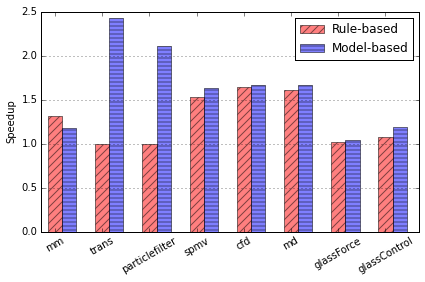
\includegraphics[width=0.6\columnwidth]{graph/dp_speedup}
	\caption{Speedup of benchmarks on Tesla K20c.}
	\label{fig:dp_speedup}
\end{figure}
%\TODO{replace PORPLE-based with model-based to contrast rule-based in the figure?}

% productivity
For productivity, PORPLE's parser for the custom MSL format written in
Python has approximately 270 lines while the ontology format can be
processed with standard libraries. The PORPLE framework is written in
an already compact scripting language, Python.  It still has about 950
lines code while the PATO implementation has about 380 lines.

% Extensibility
Compared to the alternatives, the PATO-based analyses are more
extensible and sharable due to their ontology representations and
declarative algorithms.  For example, in the previous approach used in
PORPLE, if knowledge about GPUs with new features is to be added, the
MSL format must be modified to add the corresponding fields; the code
for parsing MSL and querying the placement engine should be modified
as well.  In PATO, the changes are much easy to do. Through the Prolog
GUI, users can easily add or remove a concept. Analysis rules only
need to add queries for the features if needed.
%Besides, the PATO is more extensible in terms of productivity. For example, if a new kind of memory is added into the system, in the PORPLE, the \TODO{to be done}

%% % Overhead
%% Finally, we compare the analysis overhead of the PORPLE and PATO implementation in Figure~\ref{fig:dp_time_cmp}. 
%% The overhead is the time to run the data placement guidance algorithms, not the tested kernels. 
%% The result of \emph{glassForce} is not shown since its time is very large compared to others. 
%% The results show that the PATO's declarative implementation is comparable to the traditional imperative implementation in terms of time efficiency. 
%% The slowness is due to the overhead in PATO when the main Prolog programs call the external Python scripts calculating the cost of placement plans to answer the query \textsf{hasCost} in Listing~\ref{code:dp_model}.
%% %This overhead can be eliminated if we unify the program with one language.
%% \begin{figure}[ht]
%% 	\centering
%% 	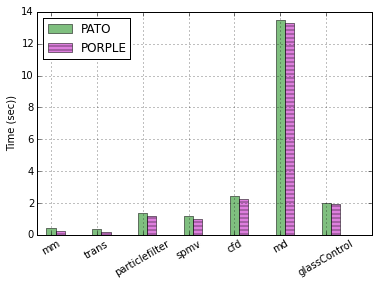
\includegraphics[width=0.7\columnwidth]{graph/dp_time_cmp}
%% 	\caption{Analysis overhead comparison}
%% 	\label{fig:dp_time_cmp}
%% \end{figure}
%% %\TODO{what is the agenda of this figure, which color is for which implementation?}

\subsection{Facilitating Cooperations}

\begin{figure}
	\centering 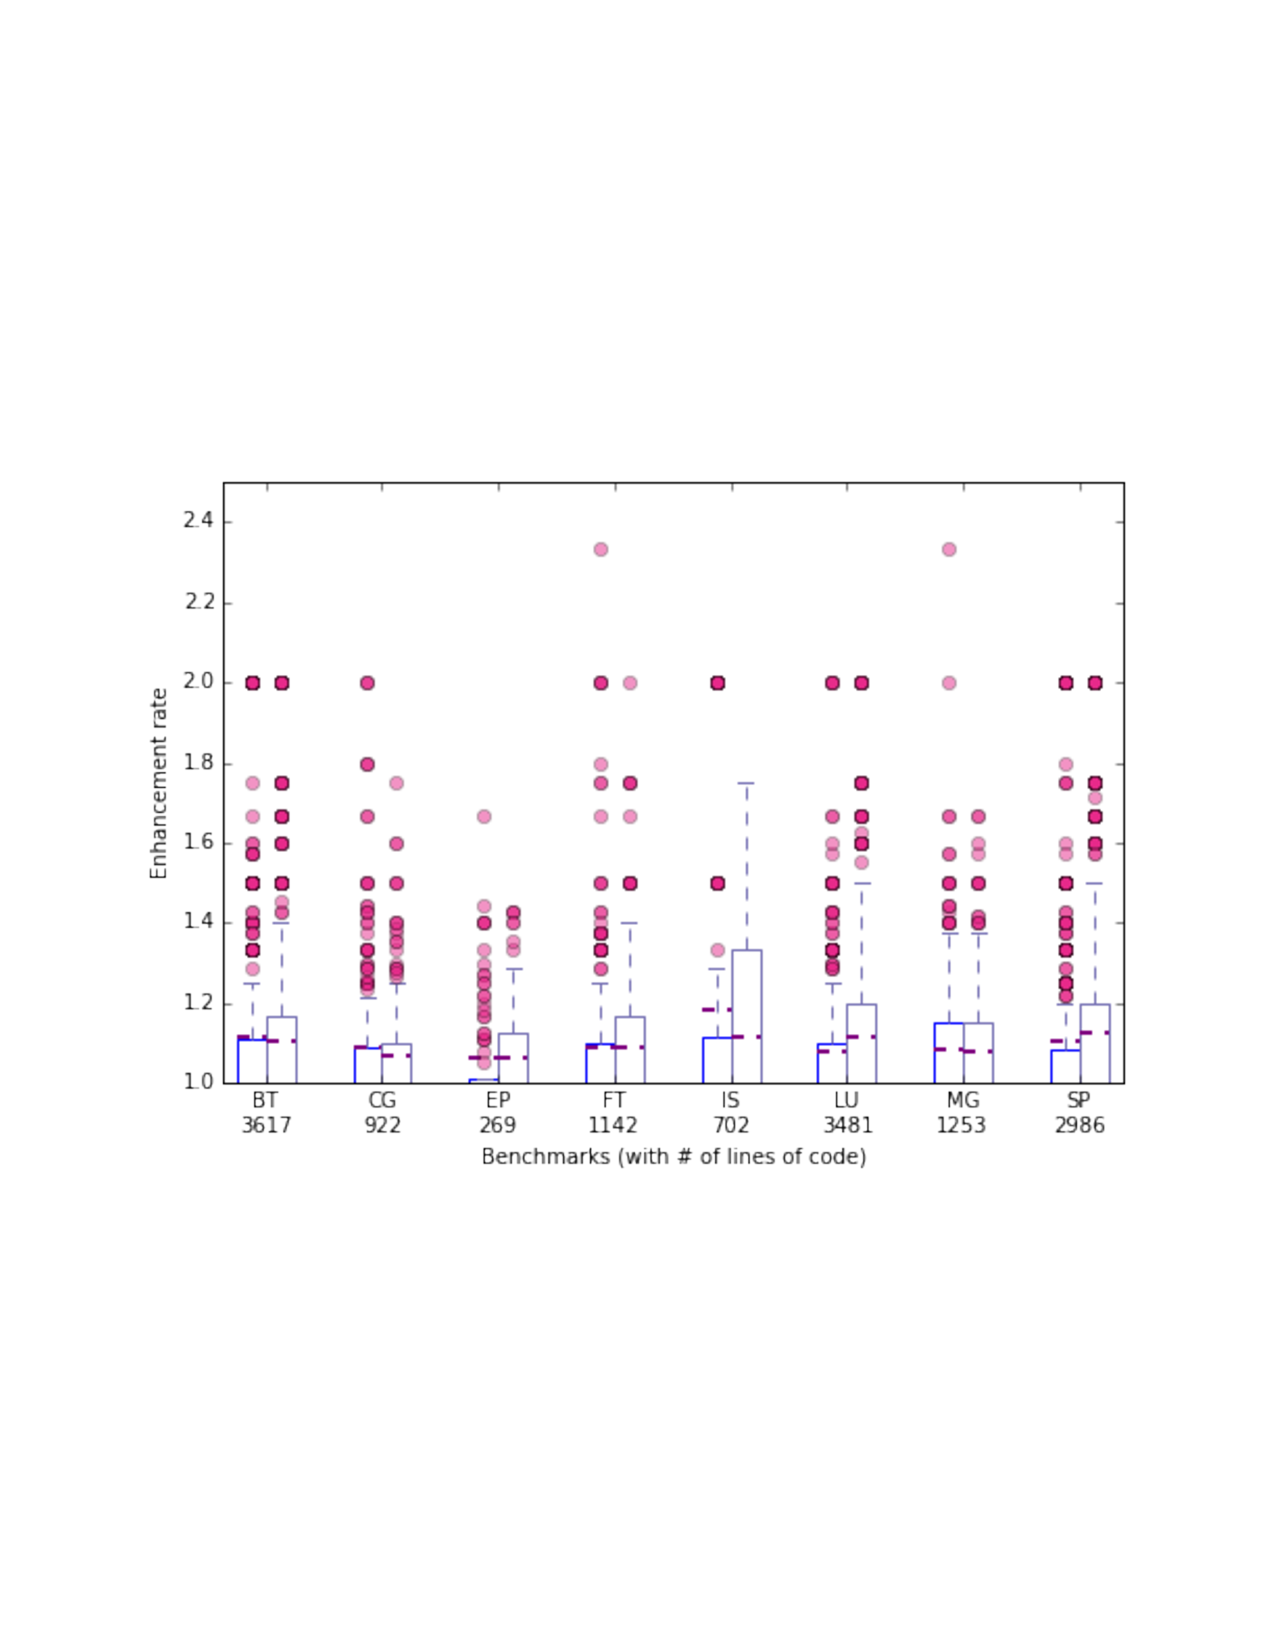
\includegraphics[width=0.6\columnwidth]{graph/lv_boxplot} \caption{Enhancement
	of Liveness analysis by leveraging ontology to combine the
	results from the Liveness analysis in LLVM Clang and
	ROSE. (Dots show outliers). Left bars: the enhancement over
	LLVM Clang results; right bars: the enhancement over ROSE
	results.}  \label{fig:coop}
\end{figure}

In the final experiment, we try to examine the potential benefits of
leveraging the standard representation of ontology to promote synergy
between different compilers. Particularly, we use Liveness analysis as
an example. 

As a {\em may-type} data flow analysis, Liveness analysis is
conservative---that is, if a variable belongs to the Liveout set of a
basic block, it means that the compiler cannot definitely tell that
the variable is dead at the end of the basic block. So, for two
different Liveness analyses (both are sound and conservative), if a
variable belongs to the result from one analysis but not that from the
other, we can conclude that that variable is not Live at the end of
the said basic block. In another word, the intersection of the results
of the two Liveness analyses gives a more precise result than either
of the two analyses. 

Both LLVM Clang and ROSE have their own Liveness analysis developed
before. By using the ontology converters we have developed for the two
compilers, we convert the Liveness analysis results from them into our
ontology. By writing several lines of Prolog code, the Prolog engine
immediately extracts out the intersection of the sets of Live
variables reported by the two compilers for each basic block of a
given program.

We define a metric called {\em enhancement rate} to characterize the
benefits of such a combination. Let A and B stand for two Liveness
analyses and $R_A$ and $R_B$ be their Liveout set for a given basic
block. The enhancement rate over $A$ is defined as

$enhancementRate(A) = \frac{|R_A|}{|R_A \cap R_B|}$

The enhancement rate over $B$ is defined similarly (with $A$ replaced with
$B$).

The results are shown in Figure~\ref{fig:coop}. Box plots are used to
show the distribution of the enhancement rates over all the basic
blocks in the program. The graph considers only the basic blocks whose
Liveout sets are not empty in the result from at least one of the two
compilers.  The results indicate that the synergy improves the average
precision of Liveness analysis by over 10\% and 20\% for LLVM Clang and ROSE
respectively.

It is worth noting that the two compilers use different internal
representations for programs and the Liveness analysis results. It is
possible to write some special code to map their results to enable
such a combination without using Ontology. However, using the ontology
designed in this work, the benefits come as simple side products of
the ontology-based program analysis (by leveraging the converters and
the standardized representation developed for many other program
analyses). The productivity benefits would become even more prominent
when many types of analyses cooperate across compilers.
